\documentclass[10pt, dvipdfmx]{beamer}
\AtBeginDvi{\special{pdf:tounicode 90ms-RKSJ-UCS2}}
\usetheme{default}
\usefonttheme{professionalfonts}
\usepackage{helvet}
\usepackage{txfonts}
\usepackage{moreverb}
% \usepackage{listings, color}
% \lstset{
%     %% language={C}, %プログラミング言語によって変える。
%     basicstyle={\ttfamily\small},
%     keywordstyle={\color{blue}},
%     commentstyle={\color{green}},
%     stringstyle=\color{red},
%     tabsize=4,
%     %% breaklines=true, %折り返し
% }
\renewcommand{\familydefault}{\sfdefault}
\renewcommand{\kanjifamilydefault}{\gtdefault}
\setbeamertemplate{caption}[numbered]

\title{Data Visualization WorkShop}
\author{}
\institute[所属]{}
\date{\today}

\uselanguage{japanese}
\languagepath{japanese}

\begin{document}
    \begin{frame}[plain]
        \frametitle{}
	    \titlepage
    \end{frame}

    \begin{frame}
        \frametitle{Contents}
        \tableofcontents
    \end{frame}

%-----------------------------------------------------------
    \section{Processingについて}
        \begin{frame}
            \frametitle{Processingとは}
            Processingとはマサチューセッツ工科大学のメディアラボが開発したデザインや映像に特化したプログラミング開発環境.
            \begin{block}{Processingの特徴}
                \begin{itemize}
                    \item 命令がとても簡単(http://ossyaritoori.hatenablog.com/entry/2016/02/16/161753)
                    \item クロスプラットフォーム(Windows, MacOS, Linux, iOSなどで動作する)
                    \item 様々な作品が生み出されている(http://www.creativeapplications.net/category/processing/)
                \end{itemize}
            \end{block}
        \end{frame}

        \begin{frame}
            \frametitle{インストール}
            Processingのウェブサイトからダウンロードする(https://processing.org/download/)
        \end{frame}

        \begin{frame}
            \frametitle{学習}
            Processingにはアプリケーションに最初からサンプルコードがプリインストールされている
            「ファイル」>「サンプル...」
        \end{frame}

        \begin{frame}
            \frametitle{参考書籍}
            \tiny
            \begin{block}{すでにたくさんの書籍が出版されています}
                \begin{itemize}
                    \item 「Processingをはじめよう」オライリージャパン 2011年
                    \item 「Processing:ビジュアルデザイナーとアーティストのためのプログラミング入門」BNN新社 2015年
                    \item 「ジェネラティブ・アート―Processingによる実践ガイド」BNN新社 2014年
                    \item 「Generative Design ―Processingで切り拓く、デザインの新たな地平」BNN新社 2016年
                    \item 「Nature of Code- Processingではじめる自然現象のシミュレーション」株式会社ボーンデジタル 2014年
                    \item 「ビジュアライジング・データ―Processingによる情報視覚化手法」オライリー・ジャパン 2008年
                    \item 「データ可視化プログラミング入門」秀和システム 2013年
                \end{itemize}
            \end{block}
        \end{frame}

%-----------------------------------------------------------
    \section{Processingの基本}
        \begin{frame}
            \frametitle{Processingの基本}
            \tiny
            \begin{columns}[c]
                \begin{column}{0.35\textwidth}
                    \begin{figure}[htb]
                        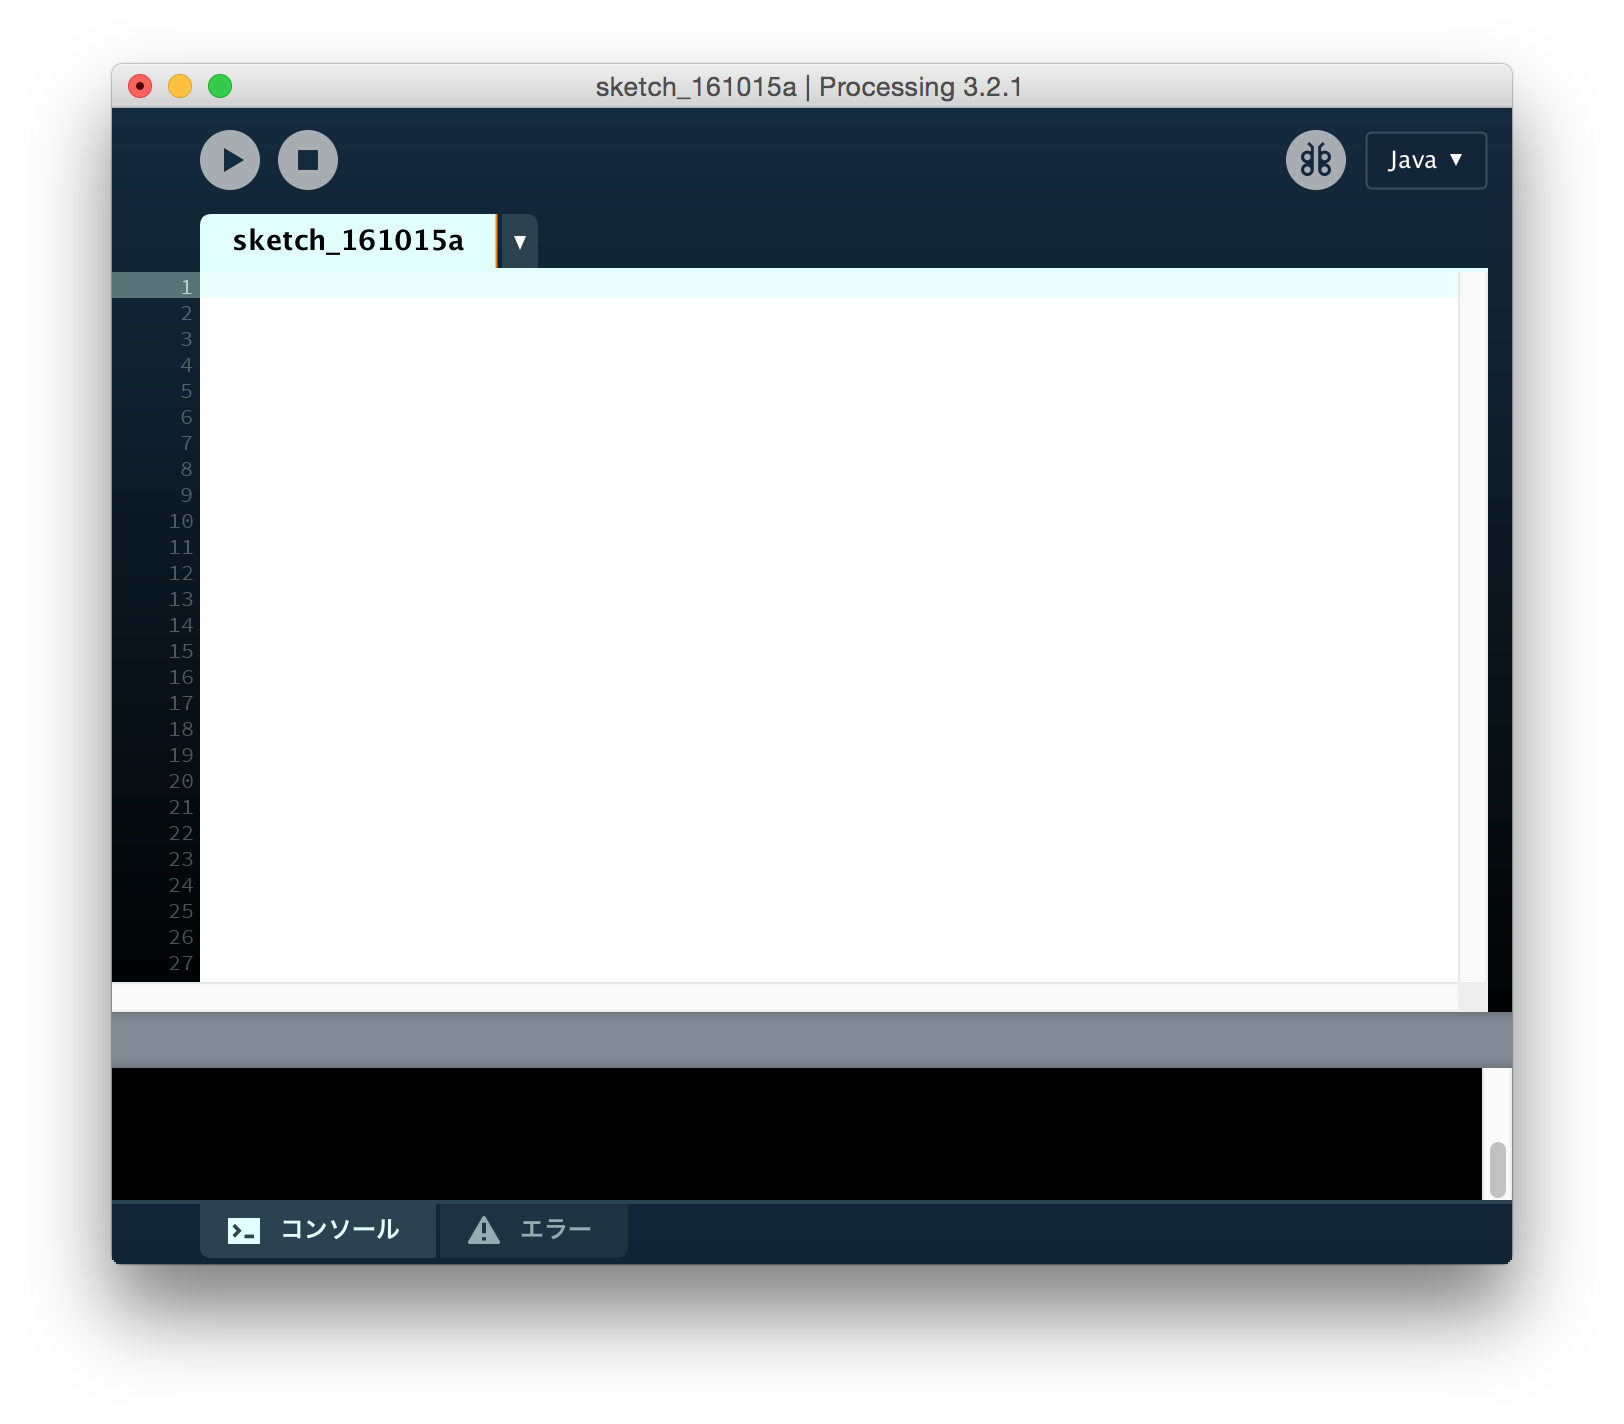
\includegraphics[width=\columnwidth]{images/01.png}
                        \caption{画面}
                        \label{fig:01}
                    \end{figure}
                \end{column}
                \begin{column}{0.20\textwidth}
                    \begin{figure}[htb]
                        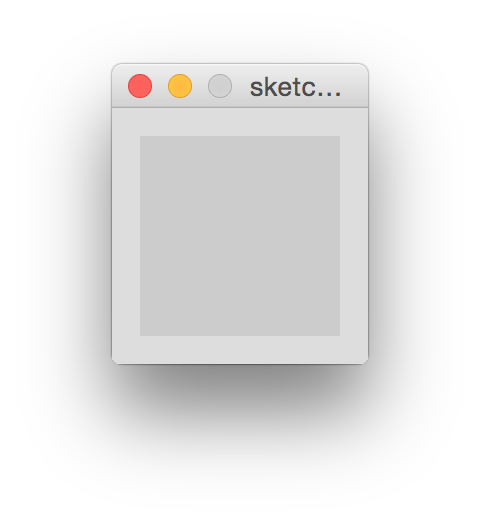
\includegraphics[width=10mm]{images/02.png}
                        \caption{結果}
                        \label{02}
                    \end{figure}
                \end{column}
                \begin{column}{0.45\textwidth}
                    \begin{block}{手順}
                        \begin{itemize}
                            \item エディタでソースコードを書く
                            \item Runボタンでスケッチを実行する
                            \item ウィンドウに描画内容が表示される
                            \item コンソールにテキストメッセージやエラーコードが表示される
                            \item Stopボタンでスケッチを停止する
                        \end{itemize}
                    \end{block}
                \end{column}
            \end{columns}
        \end{frame}

        \begin{frame}
            \frametitle{座標について}
            \Large
            Processingでは全て「ピクセル」で考えます.
        \end{frame}

% 図形を描く
        \begin{frame}
            \frametitle{円を描く}
            \begin{columns}[c]
                \begin{column}{0.50\textwidth}
                    \tiny
                    Examples/lecture/ellipse/ellipse.pde
                    \scriptsize
                    \verbatimtabinput{../Examples/lecture/ellipse/ellipse.pde}
                \end{column}
                \begin{column}{0.50\textwidth}
                    \begin{block}{楕円(ellipse)を描く.}
                        \begin{itemize}
                            \item 左から50px
                            \item 上から50px
                            \item 幅が50px
                            \item 高さが20px
                        \end{itemize}
                    \end{block}
                \end{column}
            \end{columns}
        \end{frame}

        \begin{frame}
            \frametitle{実行結果}
                \begin{figure}[htb]
                    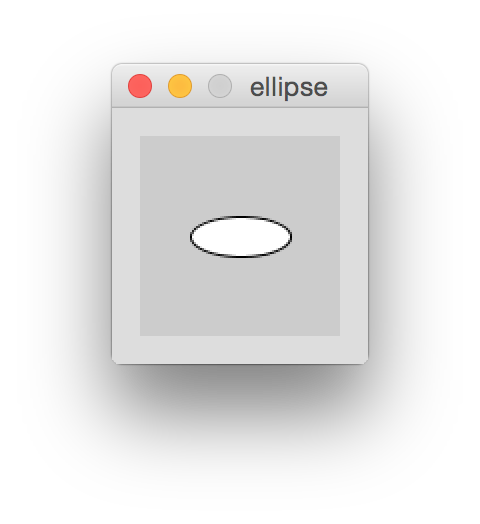
\includegraphics[width=24mm]{images/03.png}
                    \caption{楕円ができた}
                    \label{fig:03}
                \end{figure}
        \end{frame}

        \begin{frame}
            \frametitle{線を描く}
            \begin{columns}[c]
                \begin{column}{0.50\textwidth}
                    \tiny
                    Examples/lecture/line/line.pde
                    \scriptsize
                    \verbatimtabinput{../Examples/lecture/line/line.pde}
                \end{column}
                \begin{column}{0.50\textwidth}
                    \begin{block}{線(line)を描く.}
                        \begin{itemize}
                            \item 点(20, 20)から
                            \item 点(80, 80)へ
                        \end{itemize}
                    \end{block}
                \end{column}
            \end{columns}
        \end{frame}

        \begin{frame}
            \frametitle{実行結果}
                \begin{figure}[htb]
                    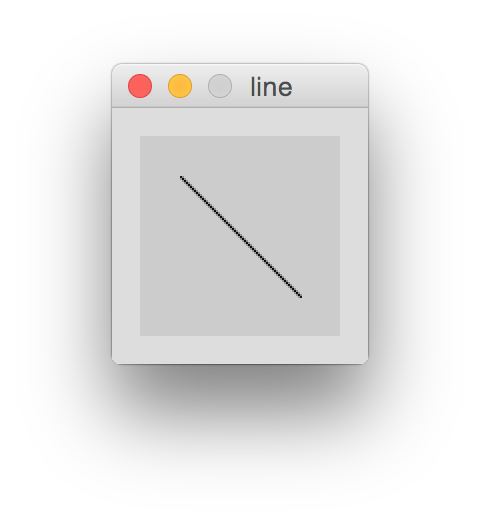
\includegraphics[width=24mm]{images/04.png}
                    \caption{線がひけた}
                    \label{fig:04}
                \end{figure}
        \end{frame}

        \begin{frame}
            \frametitle{三角形を描く}
            \begin{columns}[c]
                \begin{column}{0.50\textwidth}
                    \tiny
                    Examples/lecture/triangle/triangle.pde
                    \scriptsize
                    \verbatimtabinput{../Examples/lecture/triangle/triangle.pde}
                \end{column}
                \begin{column}{0.50\textwidth}
                    \begin{block}{三角形(triangle)を描く.}
                        \begin{itemize}
                            \item 点(01, 10)と
                            \item 点(90, 20)と
                            \item 点(60, 90)の
                        \end{itemize}
                    \end{block}
                \end{column}
            \end{columns}
        \end{frame}

        \begin{frame}
            \frametitle{実行結果}
                \begin{figure}[htb]
                    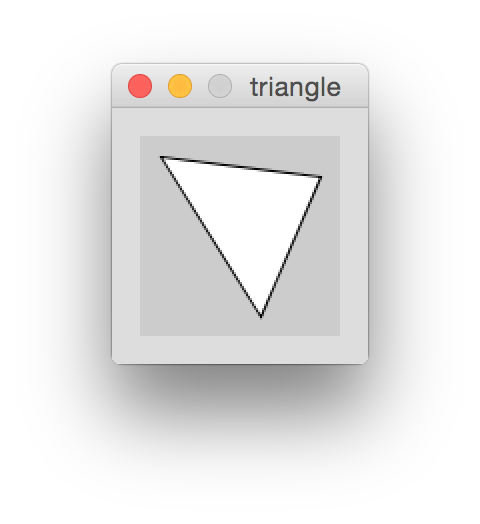
\includegraphics[width=24mm]{images/05.png}
                    \caption{三角形がかけた}
                    \label{fig:05}
                \end{figure}
        \end{frame}

        \begin{frame}
            \frametitle{四角形を描く}
            \begin{columns}[c]
                \begin{column}{0.50\textwidth}
                    \tiny
                    Examples/lecture/rect/rect.pde
                    \scriptsize
                    \verbatimtabinput{../Examples/lecture/rect/rect.pde}
                \end{column}
                \begin{column}{0.50\textwidth}
                    \begin{block}{四角形(rect)を描く.}
                        \begin{itemize}
                            \item 点(10, 10)から
                            \item 横80pxで
                            \item 縦80pxの
                        \end{itemize}
                    \end{block}
                \end{column}
            \end{columns}
        \end{frame}

        \begin{frame}
            \frametitle{実行結果}
                \begin{figure}[htb]
                    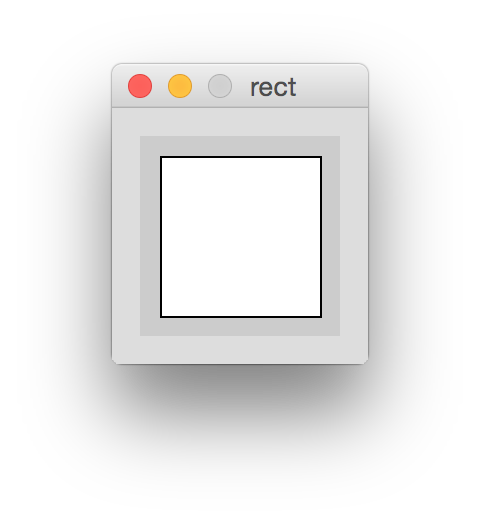
\includegraphics[width=24mm]{images/06.png}
                    \caption{四角形がかけた}
                    \label{fig:06}
                \end{figure}
        \end{frame}

% 画面サイズ
        \begin{frame}
            \frametitle{画面サイズを変える}
            \begin{columns}[c]
                \begin{column}{0.50\textwidth}
                    \tiny
                    Examples/lecture/size/size.pde
                    \scriptsize
                    \verbatimtabinput{../Examples/lecture/size/size.pde}
                \end{column}
                \begin{column}{0.50\textwidth}
                    \begin{block}{画面サイズを変更する}
                        \begin{itemize}
                            \item 横500px
                            \item 縦250pxに
                        \end{itemize}
                    \end{block}
                \end{column}
            \end{columns}
        \end{frame}

        \begin{frame}
            \frametitle{実行結果}
                \begin{figure}[htb]
                    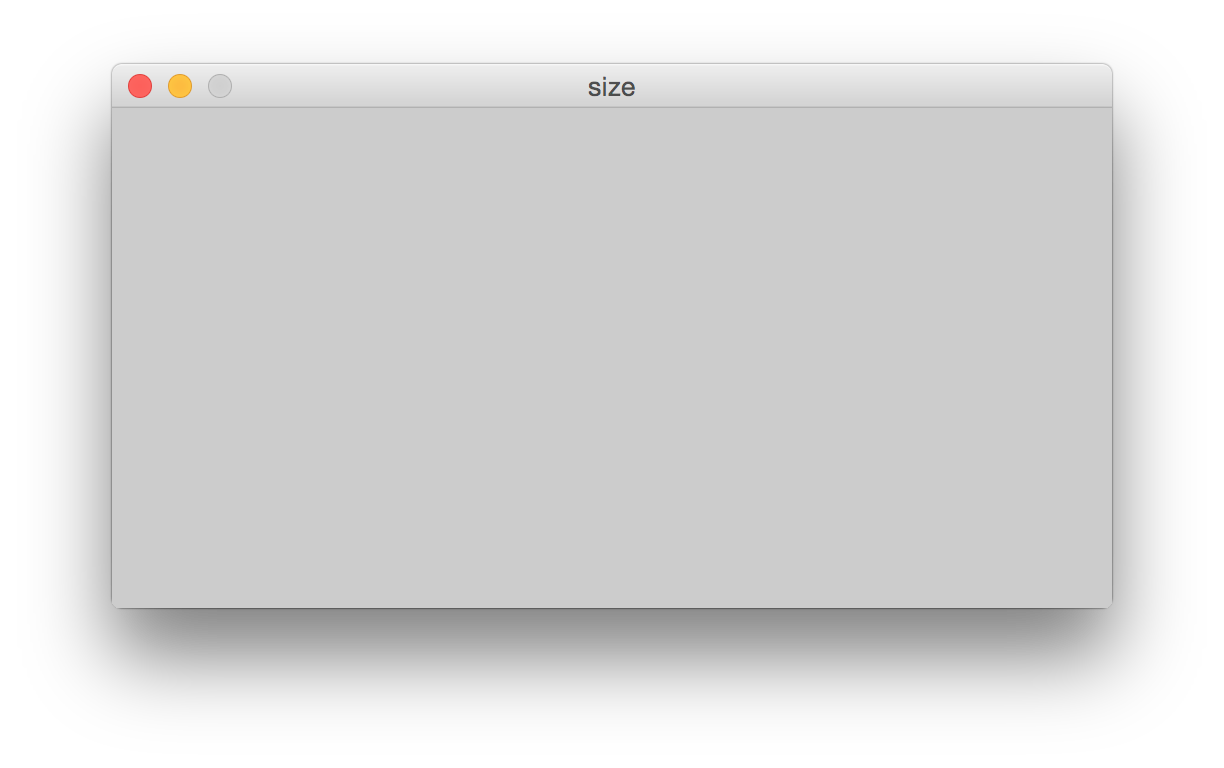
\includegraphics[width=62.1mm]{images/07.png}
                    \caption{出力サイズが変わった}
                    \label{fig:07}
                \end{figure}
        \end{frame}

% 線の太さを変える
        \begin{frame}
            \frametitle{線の太さを変える}
            \begin{columns}[c]
                \begin{column}{0.50\textwidth}
                    \tiny
                    Examples/lecture/strokeWeight/strokeWeight.pde
                    \scriptsize
                    \verbatimtabinput{../Examples/lecture/strokeWeight/strokeWeight.pde}
                \end{column}
                \begin{column}{0.50\textwidth}
                    \begin{block}{線の太さ(strokeWeight)を変える.}
                        \begin{itemize}
                            \item 線幅5pxで
                        \end{itemize}
                    \end{block}
                \end{column}
            \end{columns}
        \end{frame}

        \begin{frame}
            \frametitle{実行結果}
                \begin{figure}[htb]
                    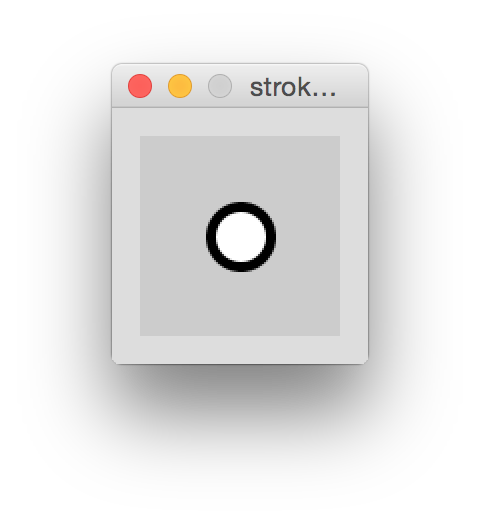
\includegraphics[width=24mm]{images/08.png}
                    \caption{線が太くなった}
                    \label{fig:08}
                \end{figure}
        \end{frame}

% 色を変える
        \begin{frame}
            \frametitle{色を変える}
            \begin{columns}[c]
                \begin{column}{0.50\textwidth}
                    \tiny
                    Examples/lecture/color/color.pde
                    \scriptsize
                    \verbatimtabinput{../Examples/lecture/color/color.pde}
                \end{column}
                \begin{column}{0.50\textwidth}
                    \begin{block}{色(stroke, fill)を変える.}
                        \begin{itemize}
                            \item 色空間をHSBで
                            \item 線色を色彩50, 彩度255, 明度255で
                            \item 塗り色を色彩122, 彩度255, 明度255で
                            \item 背景を色彩200, 彩度255, 明度255で
                            \item 線幅10pxで
                            \item 点(50, 50)から横80px. 縦80pxの円
                        \end{itemize}
                    \end{block}
                \end{column}
            \end{columns}
        \end{frame}

        \begin{frame}
            \frametitle{実行結果}
                \begin{figure}[htb]
                    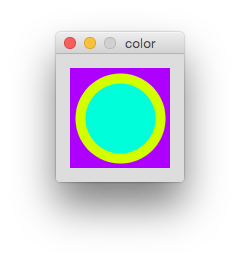
\includegraphics[width=24mm]{images/09.png}
                    \caption{色が変わった}
                    \label{fig:09}
                \end{figure}
        \end{frame}

        \begin{frame}
            \frametitle{HSB色空間}
            \begin{columns}[c]
                \begin{column}{0.50\textwidth}
                    \begin{figure}[htb]
                        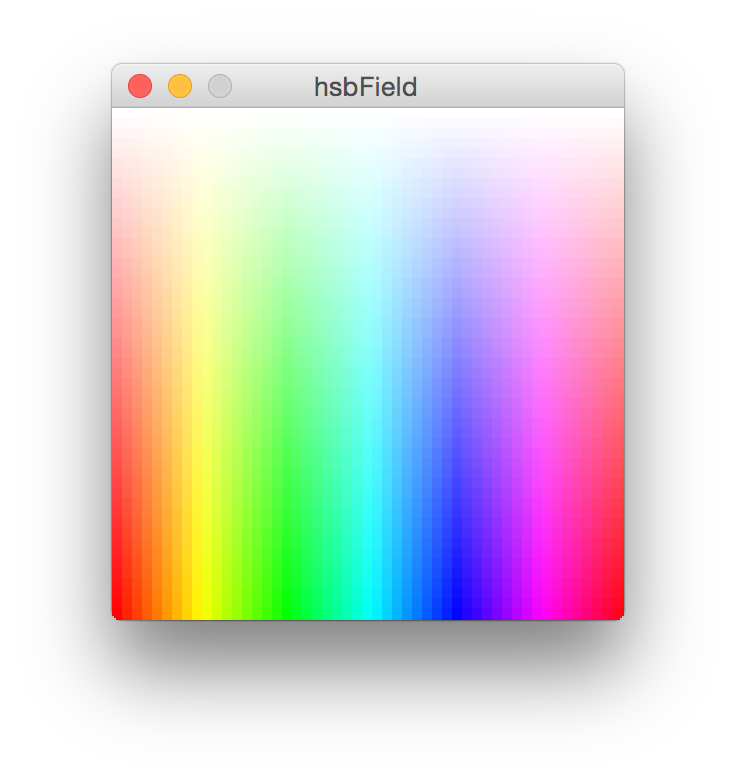
\includegraphics[width=36mm]{images/10.png}
                        \caption{HSB図(色彩 vs 彩度)}
                        \label{fig:10}
                    \end{figure}
                \end{column}
                \begin{column}{0.50\textwidth}
                    \begin{block}{色決めの指針(明度255の場合)}
                        \begin{itemize}
                            \item 色彩は左から右に0 - 255
                            \item 彩度は上から下に0 - 255
                        \end{itemize}
                    \end{block}
                \end{column}
            \end{columns}
        \end{frame}

% 型
        \begin{frame}
            \frametitle{型}
            \begin{columns}[c]
                \begin{column}{0.50\textwidth}
                    \tiny
                    Examples/lecture/type01/type01.pde
                    \scriptsize
                    \verbatimtabinput{../Examples/lecture/type01/type01.pde}
                \end{column}
                \begin{column}{0.50\textwidth}
                    \begin{block}{いろんな型}
                        \begin{itemize}
                            \item 整数
                            \item 少数
                            \item 文字列
                            \item 真偽
                            \item 点(50, 50)から横50px, 縦50pxの円?
                        \end{itemize}
                    \end{block}
                \end{column}
            \end{columns}
        \end{frame}

        \begin{frame}
            \frametitle{正しくは...}
            \begin{columns}[c]
                \begin{column}{0.50\textwidth}
                    \tiny
                    Examples/lecture/type02/type02.pde
                    \scriptsize
                    \verbatimtabinput{../Examples/lecture/type02/type02.pde}
                \end{column}
                \begin{column}{0.50\textwidth}
                    \begin{block}{キャストとは}
                        \begin{itemize}
                            \item 違う型にうつす
                            \item 文字列sを少数に
                            \item 点(50, 50)から横50px, 縦50pxの円
                        \end{itemize}
                    \end{block}
                \end{column}
            \end{columns}
        \end{frame}

        \begin{frame}
            \frametitle{実行結果}
                \begin{figure}[htb]
                    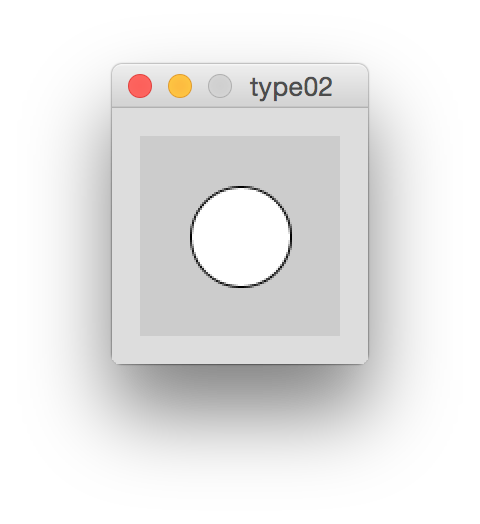
\includegraphics[width=24mm]{images/11.png}
                    \caption{円がかけた}
                    \label{fig:11}
                \end{figure}
        \end{frame}

% if文
        \begin{frame}
            \frametitle{条件文}
            \begin{columns}[c]
                \begin{column}{0.50\textwidth}
                    \tiny
                    Examples/lecture/joken/joken.pde
                    \scriptsize
                    \verbatimtabinput{../Examples/lecture/joken/joken.pde}
                \end{column}
                \begin{column}{0.50\textwidth}
                    \begin{block}{if文}
                        \begin{itemize}
                            \item 比較演算子いろいろで数字を比較
                            \item if(xxxx) 文.xxxは真偽
                        \end{itemize}
                    \end{block}
                \end{column}
            \end{columns}
        \end{frame}

% for文
        \begin{frame}
            \frametitle{繰り返し}
            \begin{columns}[c]
                \begin{column}{0.50\textwidth}
                    \tiny
                    Examples/lecture/loop/loop.pde
                    \scriptsize
                    \verbatimtabinput{../Examples/lecture/loop/loop.pde}
                \end{column}
                \begin{column}{0.50\textwidth}
                    \begin{block}{for文}
                        \begin{itemize}
                            \item 0 から 9 まで
                            \item カッコ内の処理を繰り返す
                        \end{itemize}
                    \end{block}
                \end{column}
            \end{columns}
        \end{frame}

        \begin{frame}
            \frametitle{実行結果}
                \begin{figure}[htb]
                    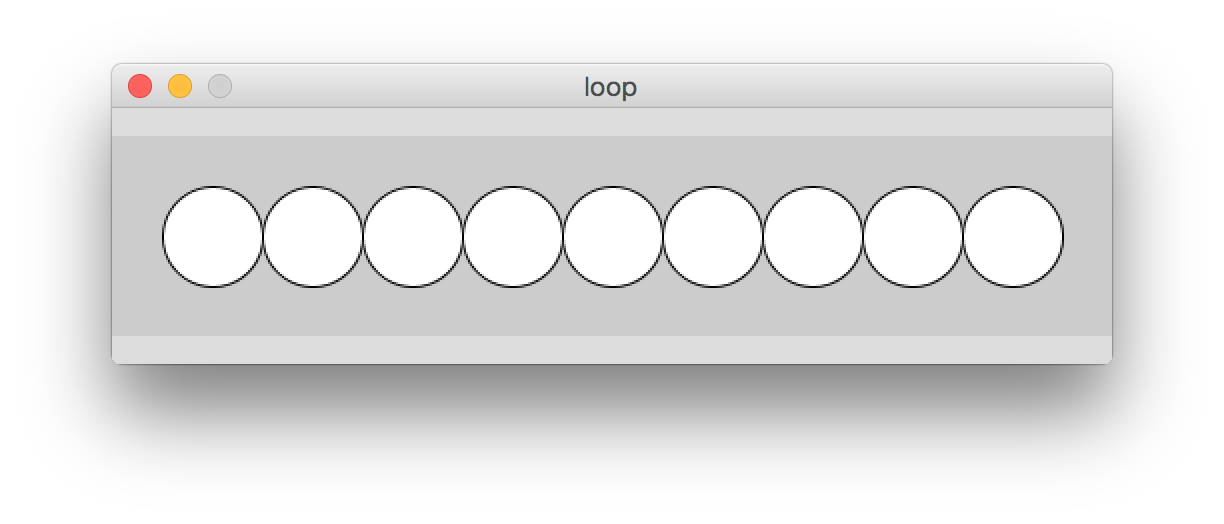
\includegraphics[width=61mm]{images/12.png}
                    \caption{円が10個かけた}
                    \label{fig:12}
                \end{figure}
        \end{frame}

% 配列
        \begin{frame}
            \frametitle{配列}
            \begin{columns}[c]
                \begin{column}{0.50\textwidth}
                    \tiny
                    Examples/lecture/array/array.pde
                    \scriptsize
                    \verbatimtabinput{../Examples/lecture/array/array.pde}
                \end{column}
                \begin{column}{0.50\textwidth}
                    \begin{block}{配列}
                        \begin{itemize}
                            \item nという5つの箱(配列)を準備
                            \item for文のなかで,0から4番目の箱に値を入れる
                        \end{itemize}
                    \end{block}
                \end{column}
            \end{columns}
        \end{frame}

 % サンプルプログラムをみる
        \begin{frame}
            \frametitle{}
            \centering
            \large
            それではサンプルプログラムを見てみましょう.
        \end{frame}

% CSVの値の指定
        \begin{frame}
            \frametitle{CSVデータの指定}
            \begin{columns}[c]
                \begin{column}{0.50\textwidth}
                    \begin{figure}[htb]
                        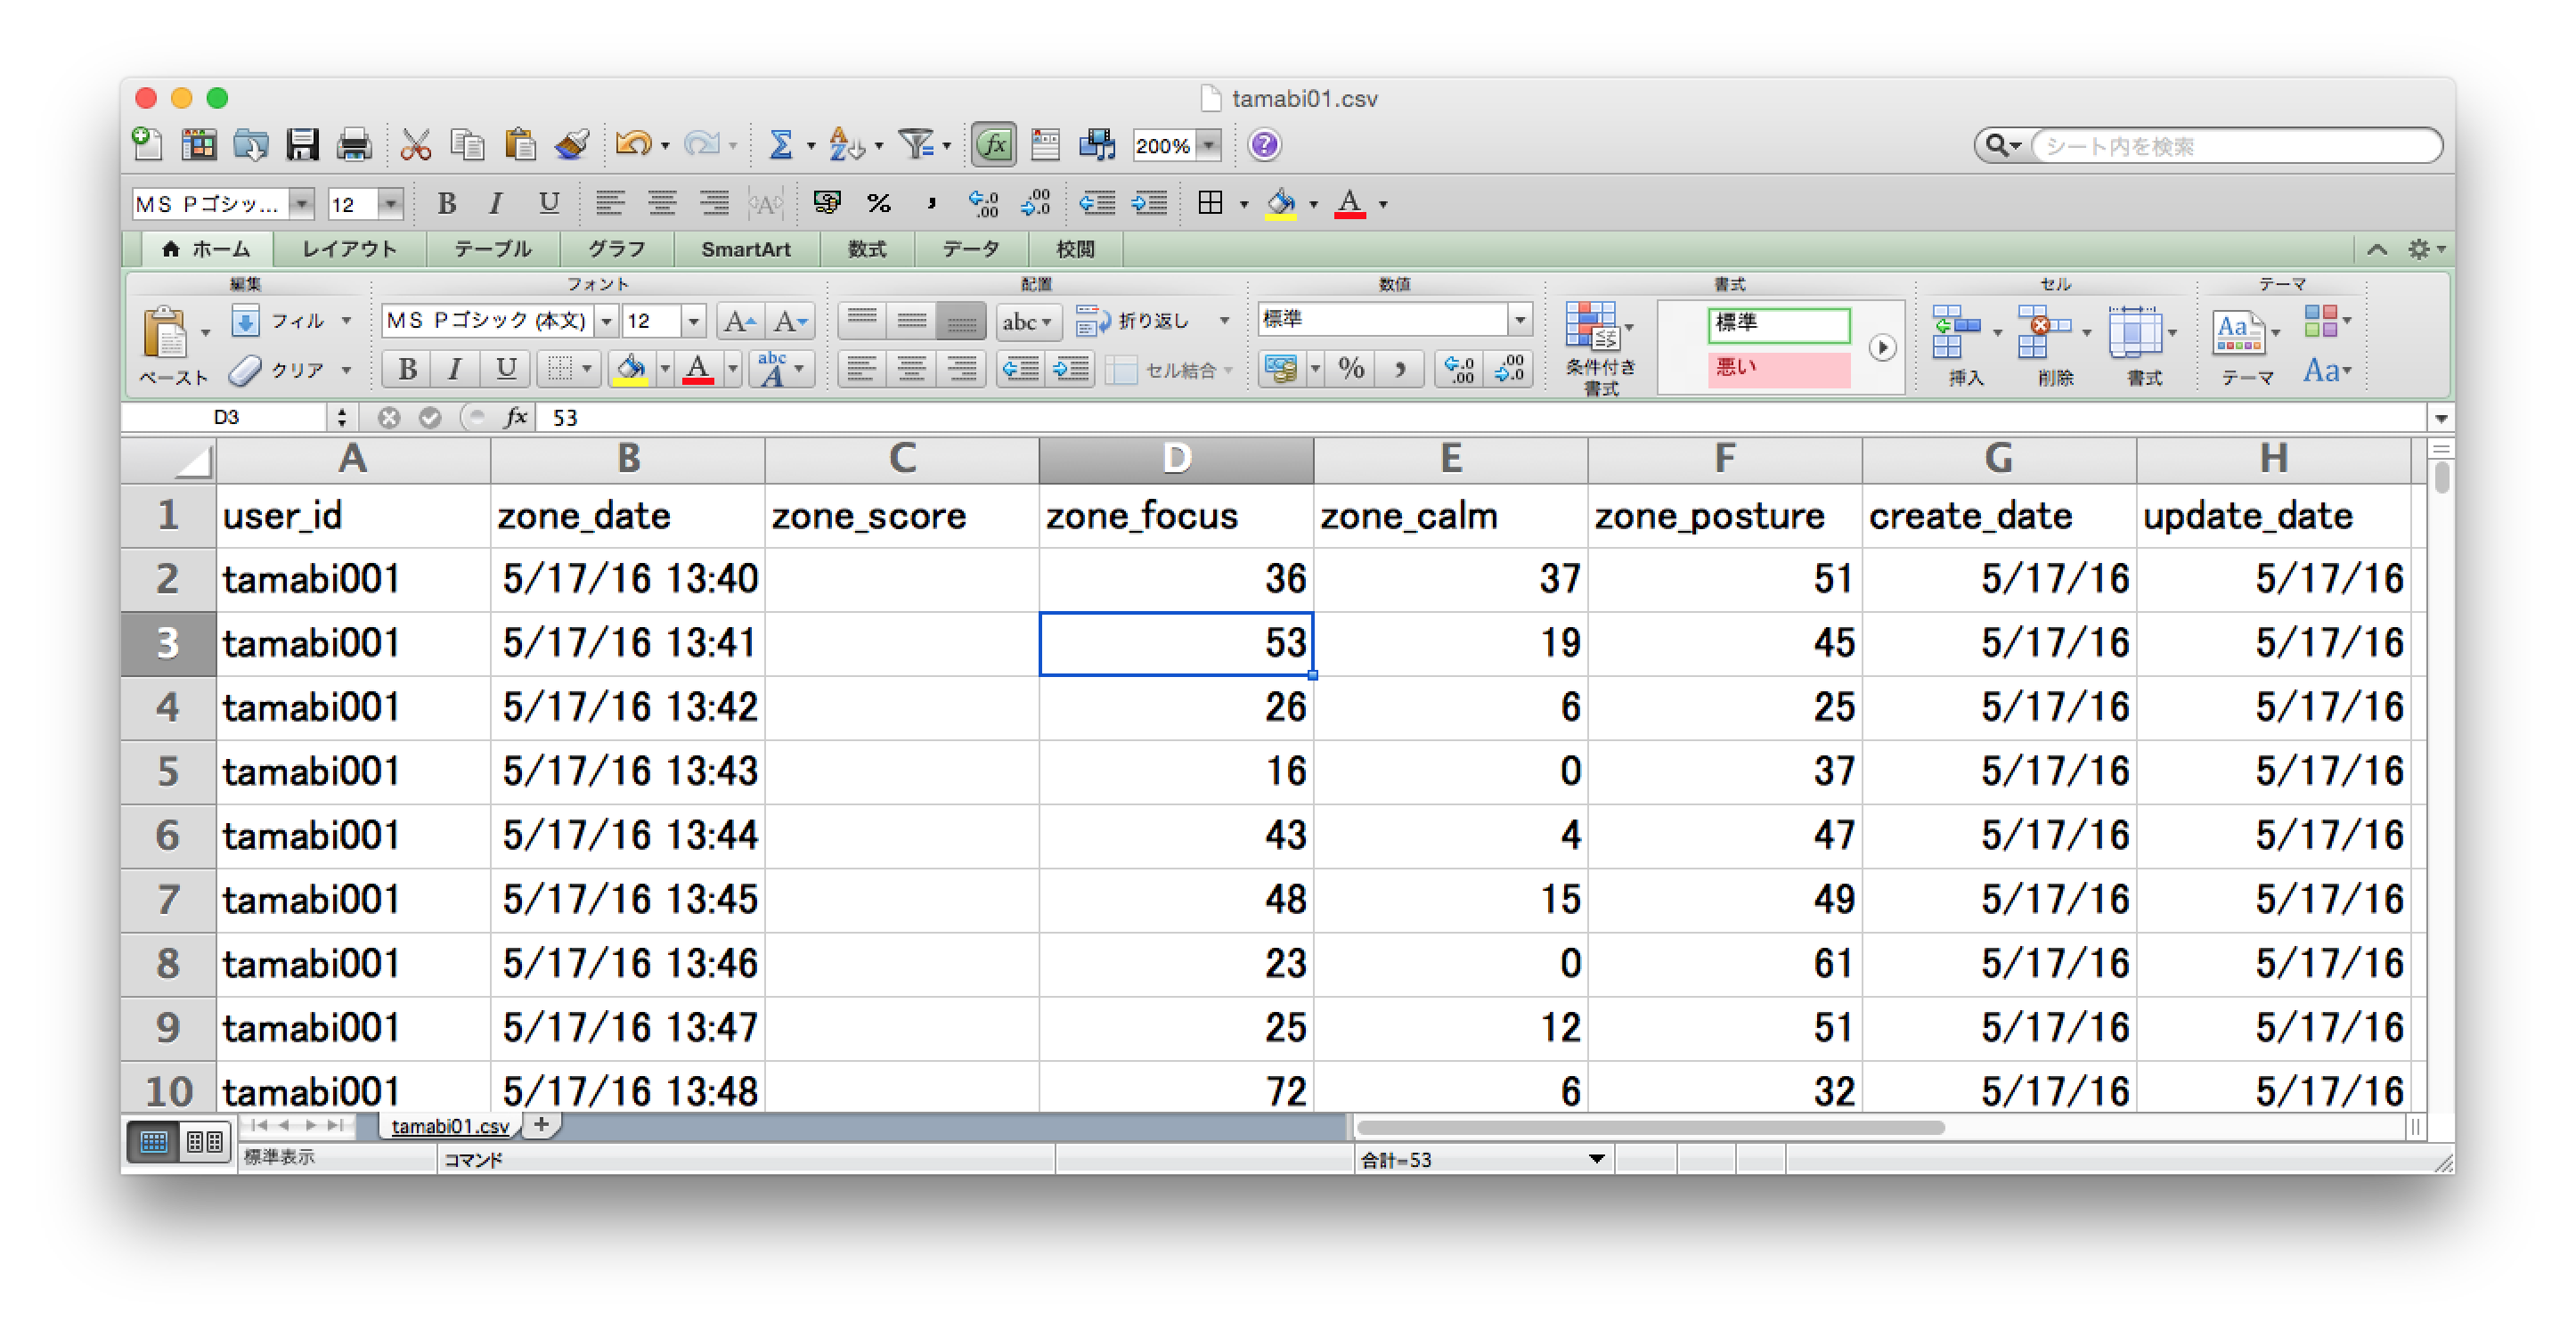
\includegraphics[width=50mm]{images/13.png}
                        \caption{CSV中身}
                        \label{fig:13}
                    \end{figure}
                \end{column}
                \begin{column}{0.50\textwidth}
                    \begin{block}{指定の仕方}
                        \begin{itemize}
                            \tiny
                            \item i は誰のデータか(0 - 17番目までの18名分)
                            \item j はCSVの何列目か
                            \item k は何行目か
                            \item 図の場合は「data[0][3][2]」
                            \item 同じ人の違う項目は「j」を変える
                            \item 違う人の同じ項目は「i」を変える
                        \end{itemize}
                    \end{block}
                \end{column}
            \end{columns}
        \end{frame}


\end{document}


